% Visualization Code for Overleaf (TikZ / PGFPlots)

% Preamble required locally:
% \usepackage{tikz}
% \usepackage{pgfplots}
% \pgfplotsset{compat=1.17}
% \usetikzlibrary{shapes,arrows,positioning,calc}

% ==================================================
% Figure 1: Conceptual Comparison (Trap Avoidance)
% ==================================================
\begin{figure}[h]
\centering
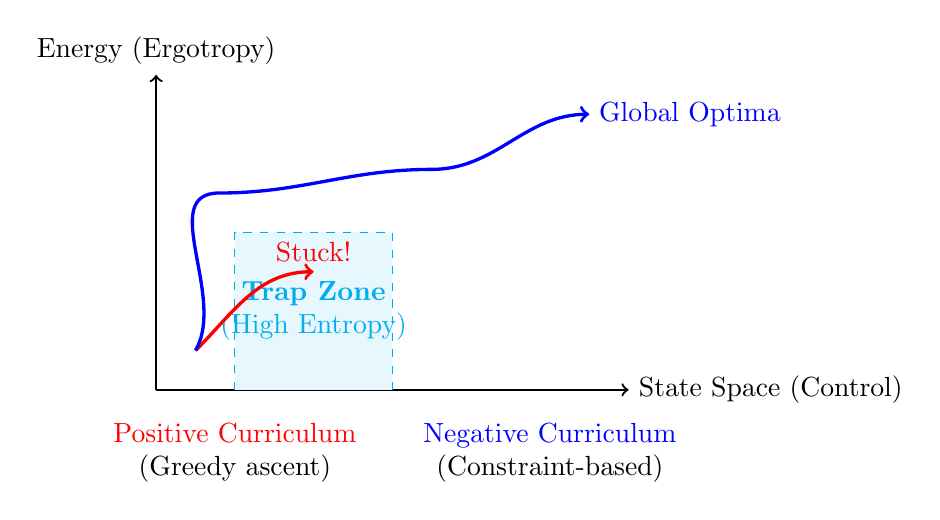
\begin{tikzpicture}[scale=1.0, transform shape]
    % Axes
    \draw[thick, ->] (0,0) -- (6,0) node[right] {State Space (Control)};
    \draw[thick, ->] (0,0) -- (0,4) node[above] {Energy (Ergotropy)};
    
    % Trap Region (Cyan Rectangle)
    \fill[cyan!10] (1,0) rectangle (3, 2);
    \draw[cyan, dashed] (1,0) -- (1,2) -- (3,2) -- (3,0);
    \node[cyan, align=center] at (2, 1) {\textbf{Trap Zone}\\(High Entropy)};
    
    % Positive Curriculum Path (Red) - Goes into Trap
    \draw[red, very thick, ->] (0.5,0.5) to[out=45,in=180] (2,1.5);
    \node[red, above] at (2,1.5) {Stuck!};
    
    % Negative Curriculum Path (Blue) - Avoids Trap
    \draw[blue, very thick, ->] (0.5,0.5) 
        to[out=60,in=180] (0.8, 2.5) 
        to[out=0,in=180] (3.5, 2.8) 
        to[out=0,in=180] (5.5,3.5);
    \node[blue, right] at (5.5,3.5) {Global Optima};
    
    % Labels
    \node[align=center] at (1,-0.8) {\textcolor{red}{Positive Curriculum}\\(Greedy ascent)};
    \node[align=center] at (5,-0.8) {\textcolor{blue}{Negative Curriculum}\\(Constraint-based)};
\end{tikzpicture}
\caption{Conceptual diagram: Positive Curriculum gets trapped in local optima (entropy cliffs), while Negative Curriculum navigates around forbidden zones to reach the true peak.}
\end{figure}

% ==================================================
% Figure 2: Learning Curves (Results)
% ==================================================
\begin{figure}[h]
\centering
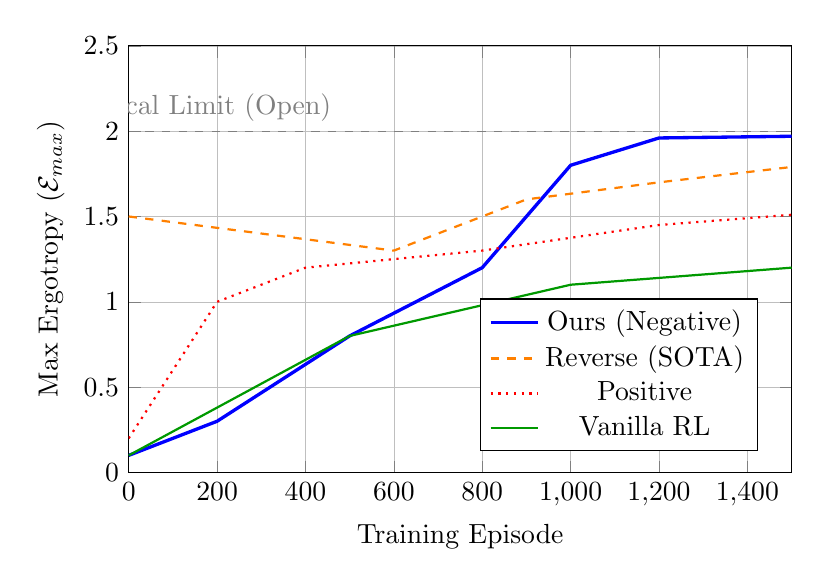
\begin{tikzpicture}
\begin{axis}[
    width=10cm, height=7cm,
    xlabel={Training Episode},
    ylabel={Max Ergotropy ($\mathcal{E}_{max}$)},
    legend style={at={(0.95,0.05)},anchor=south east},
    grid=both,
    grid style={line width=.1pt, draw=gray!10},
    major grid style={line width=.2pt,draw=gray!50},
    xmin=0, xmax=1500,
    ymin=0, ymax=2.5
]
    % Ours (Negative) - Hypothetical Smooth Data
    \addplot[color=blue, very thick, mark=none] coordinates {
        (0,0.1) (100, 0.2) (200, 0.3) % Stage 1 (Low energy but safe)
        (500, 0.8) (800, 1.2)         % Stage 2 (Purity maintenance)
        (1000, 1.8) (1200, 1.96) (1500, 1.97) % Stage 3 (Exploration)
    };
    \addlegendentry{Ours (Negative)}
    
    % Reverse Curriculum (SOTA)
    \addplot[color=orange, thick, dashed] coordinates {
        (0,1.5) (300, 1.4) (600, 1.3) % Starts high (reverse)
        (900, 1.6) (1200, 1.7) (1500, 1.79)
    };
    \addlegendentry{Reverse (SOTA)}
    
    % Positive Curriculum
    \addplot[color=red, thick, dotted] coordinates {
        (0,0.2) (200, 1.0) (400, 1.2) % Quick rise
        (800, 1.3) (1200, 1.45) (1500, 1.51) % Stuck
    };
    \addlegendentry{Positive}
    
    % Vanilla
    \addplot[color=green!60!black, thick] coordinates {
        (0,0.1) (500, 0.8) (1000, 1.1) (1500, 1.20)
    };
    \addlegendentry{Vanilla RL}
    
    % Theoretical Max line
    \draw [red, dashed] (axis cs:0,4.0) -- (axis cs:1500,4.0) node [pos=0.5, above] {Theoretical Max (Closed)};
    \draw [gray, dashed] (axis cs:0,2.0) -- (axis cs:1500,2.0) node [pos=0.1, above] {Physical Limit (Open)};
\end{axis}
\end{tikzpicture}
\caption{Learning performance comparison. Ours (Blue) initially learns slowly (safety first) but accelerates in later stages to surpass all baselines.}
\end{figure}
